\documentclass{beamer}
\usepackage{pgfplots}

\beamertemplatenavigationsymbolsempty{}

\title{Optimization of a Distributed Storage Architecture under Uncertain
Demand}
\subtitle{A Study in Fast Flow Algorithms}
\date{March 20, 2015}

\author{Paul Beaujean\inst{*}\inst{\dag} \and \'Eric Gourdin\inst{\dag}}
\institute{\inst{*}ENSIIE-MPRO \and \inst{\dag}Orange Labs}

\begin{document}

\frame{\titlepage}

\begin{frame}
    \frametitle{Table of Contents}
    \tableofcontents{}
\end{frame}

\begin{frame}
    \frametitle{Context: Increase in IP Video}

    \begin{block}{The rise of IP video}
        \begin{itemize}
            \item Increase in IP video traffic over the past few years.
            \item Believed to amount for 80\% of all IP traffic by 2020.
        \end{itemize}
    \end{block}

    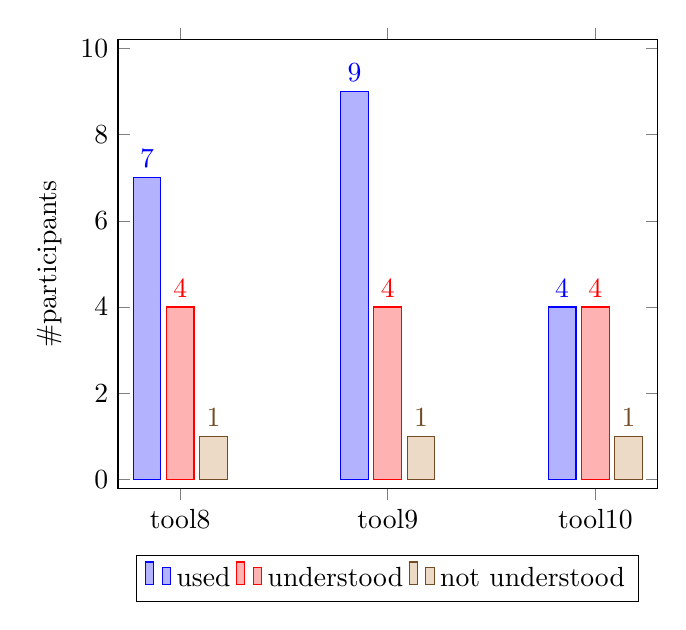
\begin{tikzpicture}
        \begin{axis}[
            ybar,
            enlargelimits=0.15,
            legend
            style={at={(0.5,-0.15)},
            anchor=north,legend columns=-1},
            ylabel={\#participants},
            symbolic x coords={tool8,tool9,tool10},
            xtick=data,
            nodes near coords,
            nodes near coords align={vertical},
            ]
            \addplot coordinates {(tool8,7) (tool9,9) (tool10,4)};
            \addplot coordinates {(tool8,4) (tool9,4) (tool10,4)};
            \addplot coordinates {(tool8,1) (tool9,1) (tool10,1)};
            \legend{used,understood,not understood}
        \end{axis}
    \end{tikzpicture}
    Insert nice picture from Cisco Visual Networking Index, hopefully TikZ?

\end{frame}

\begin{frame}
    \frametitle{Content Delivery Network}

    A Content Delivery Network is a distributed storage architecture.

    Provides content to users by caching it close to where it is requested.

    Less upstream bandwidth consumption.
\end{frame}

\begin{frame}
    \frametitle{Content Delivery = Multicommodity Flow}

    Insert a beautiful picture of multiple servers delivering contents to
    multiple clients.

\end{frame}

\begin{frame}
    \frametitle{Fractional Multiflow is in P}
    
    A peculiar problem that does not admit a combinatorial algorithm.

    In P because it can be solved with IPM on a poly-size edge formulation.

\end{frame}

\begin{frame}
    \frametitle{Too large of a LP}

    Prohibitively expensive. (cue to Sourour's $n^3$ trick)

    Solving it in practice with a exponential-size path formulation.
\end{frame}

\begin{frame}
    \frametitle{Column Generation with the path formulation}
    
    Column generation is a version of the simplex algorithm without an implicit 
    tableau.
    
    Pivot rule // Separation oracle // Shortest path problem.

    Simplex algorithm: no worst-case poly-time guarantee

\end{frame}

\begin{frame}
    \frametitle{Designing a combinatorial FPTAS}

    Different approach: poly-time combinatorial algorithm but
    $\epsilon$-approximate solution.

    FPTAS An algorithm that provides a solution within an arbitrary
    approximation guarantee and runs in time bounded by a polynomial in the
    instance size and in the approximation guarantee.

\end{frame}

\begin{frame}
    \frametitle{Learning from experts}

    Actions

    Gain

    Weights

\end{frame}

\begin{frame}
    \frametitle{A surprising result: bounded regret}

    $G \geq G_a - \epsilon |G_a| - \frac{\ln |A|}{\epsilon}, \forall a \in A$
\end{frame}

\begin{frame}
    \frametitle{Mapping multiplicative weights concepts to multiflow}
\end{frame}

\begin{frame}
    \frametitle{Combining regret bounds and flow on shortest paths}

\end{frame}

\begin{frame}
    \frametitle{Numerical experiments}

\end{frame}

\begin{frame}
    \frametitle{Conclusion}

    CDN design gives a strong incentive to study multiflow.

    Interesting alternative to exact resolution.


\end{frame}


\end{document}
